\documentclass[border=5pt]{standalone}
\usepackage{tikz}
\usepackage{amsmath}
\usetikzlibrary{arrows.meta, positioning, shapes.geometric}

\begin{document}
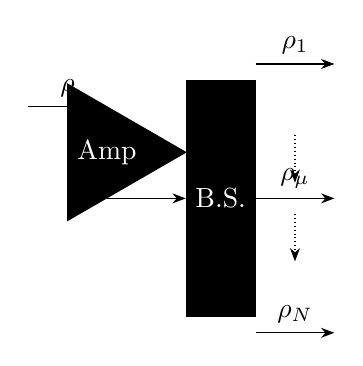
\begin{tikzpicture}[
  >=Stealth,
  box/.style={rectangle, draw, fill=black, minimum width=0.8cm, minimum height=3cm},
  amp/.style={regular polygon, regular polygon sides=3, draw, fill=black, 
              minimum width=1.5cm, minimum height=2cm},
  dotted arrow/.style={->, densely dotted},
  solid arrow/.style={->},
]

% 放大器
\node[amp, rotate=-90] (amp) at (0,0) {};
\node[white] at (amp) {Amp};

% 分束器
\node[box, right=1cm of amp] (bs) {B.S.};
\node[white] at (bs) {B.S.};

% 输入箭头和标签
\draw[solid arrow] ([xshift=-1cm]amp.west) -- (amp.west) node[midway, above] {$\rho$};

% 放大器到分束器的连接
\draw[solid arrow] (amp.east) -- (bs.west);

% 输出箭头和标签
\draw[solid arrow] (bs.east) -- ++(1cm,0) node[midway, above] {$\rho_\mu$};

% 顶部输出
\draw[solid arrow] ([yshift=0.2cm]bs.north east) -- ++(1cm,0) node[midway, above] {$\rho_1$};

% 底部输出
\draw[solid arrow] ([yshift=-0.2cm]bs.south east) -- ++(1cm,0) node[midway, above] {$\rho_N$};

% 虚线表示省略
\draw[dotted arrow] ([xshift=0.5cm, yshift=0.8cm]bs.east) -- ([xshift=0.5cm, yshift=0.2cm]bs.east);
\draw[dotted arrow] ([xshift=0.5cm, yshift=-0.2cm]bs.east) -- ([xshift=0.5cm, yshift=-0.8cm]bs.east);

\end{tikzpicture}
\end{document}